
\serie{Lecture de tableaux}

\begin{exercice}[Promenons‑nous dans les bois]
Dans le bois, j'ai fait le relevé suivant : trois‑cent‑vingt arbres sont des chênes, cent‑vingt arbres sont des hêtres et j'ai compté quarante sapins. Recopie et complète le tableau :
 \begin{center}
 \renewcommand*\tabularxcolumn[1]{>{\centering\arraybackslash}m{#1}}
 \begin{ttableau}{\linewidth}{5}
  \hline
  & \cellcolor{H2} Chênes & \cellcolor{H2} Hêtres & \cellcolor{H2} Sapins & \cellcolor{H2} Total \\\hline
  \rowcolor{H2} Nombre & & & & \\\hline
  \end{ttableau}
\end{center}
\end{exercice}


\begin{exercice}[Regrouper des notes]
Voici les points obtenus dans un test de mathématiques :

12 ; 10 ; 11 ; 12 ; 14 ; 19 ; 10 ; 15 ; 20 ; 09 ; 18 ; 14 ; 12 ; 11 ; 12 ; 11 ; 11 ; 08 ; 10 ; 14.
\begin{enumerate}
 \item Combien d'élèves ont obtenu 10 points ou moins ?
 \item Combien d'élèves ont obtenu entre 11 et 15 points ?
 \item Combien d'élèves ont obtenu 16 points ou plus ?
 \end{enumerate}
\end{exercice}


\begin{exercice}[Facture]
 Voici un extrait d'une facture téléphonique :
 \begin{center}
 \begin{tabularx}{\linewidth}{|l|X|X|X|}
  \hline
  & \cellcolor{J1} Prix HT en CHF & \cellcolor{J1} TVA  en CHF & \cellcolor{J1} Prix TTC en CHF \\\hline
 \cellcolor{J1} Abonnement & \cellcolor{J3} 29,26 & \cellcolor{J3} 5,73 & \cellcolor{J3} A  \\\hline
 \cellcolor{J1} Consommation &  \cellcolor{J3} 7,98 &  \cellcolor{J3} B &  \cellcolor{J3} 9,54  \\\hline
  \end{tabularx}
 \end{center}
Le montant TTC (toutes taxes comprises) s'obtient en additionnant la TVA au montant HT (hors taxes).
\begin{enumerate}
 \item Quelles sont les valeurs de $A$ et $B$ ? Justifie.
 \item Donne un ordre de grandeur du montant total nécessaire pour régler cette facture.
 \end{enumerate}
\end{exercice}


\begin{exercice}[Horaires]
Voici un extrait d'horaires du RER :
 \begin{center}
 \begin{tabularx}{\linewidth}{|c|X|X|X|X|X|}
  \hline
   & \cellcolor{A3} \quad \rotatebox{90}{RER 1} & \cellcolor{A3} \quad \rotatebox{90}{RER 2} & \cellcolor{A3} \quad \rotatebox{90}{RER 3} & \cellcolor{A3} \quad \rotatebox{90}{RER 4} & \cellcolor{A3} \quad \rotatebox{90}{RER 5} \\\hline
  \rowcolor{A4} Coppet & 7.22 & 8.12 & 9.10 & 18.45 & 20.14 \\\hline
  \rowcolor{A3} Mies & 7.32 & 8.20 & 9.18 & & 20.23 \\\hline
  \rowcolor{A4} Versoix & 7.40 & 8.27 & 9.25 & 18.59 & 20.30 \\\hline
  \rowcolor{A3} Genève & 7.57 & 8.41 & 9.45 & & 20.44 \\\hline
  \rowcolor{A4} Vernier & 8.07 & 8.50 & 9.56 & & 20.53 \\\hline
  \rowcolor{A3} Russin & 8.20 & 9.03 & 10.09 & & 21.06 \\\hline
  \rowcolor{A4} La Plaine & & 9.22 & & & \\\hline
  \rowcolor{A3} Bellegarde & 8.44 & 9.30 & 10.32 & 19.56 & 21.29 \\\hline
  \end{tabularx}
\end{center}
\begin{enumerate}
 \item Que signifient les cases vides du tableau ?
 \item Malika veut arriver à Bellegarde avant 10 h. Elle part de Vernier. Quel(s) train(s) peut‑elle choisir ?
 \item Finalement, elle prend le train de 8 h 50. Quelle est la durée du trajet ?
 \item Sébastien part de Coppet après 18 h pour aller à Bellegarde. Il décide de prendre le train le plus rapide. Quel train va‑t‑il choisir ?
 \end{enumerate}
\end{exercice}

%%%%%%%%%%%%%%%%%%%%%%%%%%%%%%%%%%%%%%%%%%%%%%%%%%%%%%%%%%%%%%%%%%%%%%%%%%%%%%

\serie{Lecture de graphiques}

\begin{exercice}[Températures]
Températures relevées un jour de juillet 2008 à Sion :
\begin{center} 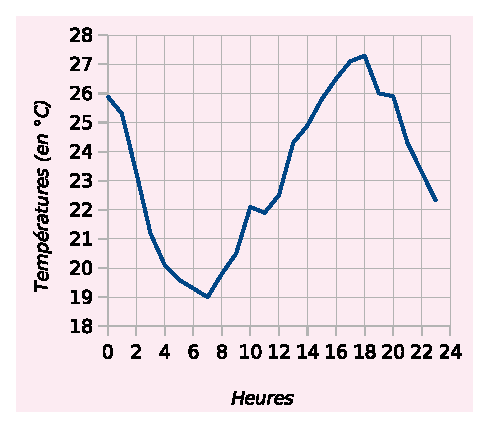
\includegraphics[width=8cm]{temperatures} \end{center}
\begin{enumerate}
 \item Quelle température faisait‑il à 4 h ?
 \item Quand a‑t‑il fait $25^\circ$C ?
 \item À quelle période de la journée la température est‑elle la plus élevée ? La plus basse ?
 \end{enumerate}
\end{exercice}

%%%%%%%%%%%%%%%%%%%%%%%%%%%%%%%%%%%%%%%%%%%%%%%%%%%%%%%%%%%%%%%%%%%%%%%%%%%%%%

\serie{Interprétation}

\begin{exercice}[Langue vivante]
Un collège compte 240 élèves. Les élèves sont, soit demi‑pensionnaires (D.P.), soit externes. Chacun de ces élèves étudie une 2\up{ème} langue au choix : anglais, allemand ou espagnol. \\[0.5em]
Quelles sont les valeurs de $A$, $B$, $C$, $D$, $E$, $F$, $G$ ? Justifie.
 \begin{center}
 \begin{tabular}{|c|c|c|c|c|}
  \hline
  & \cellcolor{A3} \small{Anglais} & \cellcolor{A3} \small{Allemand} & \cellcolor{A3} \small{Espagnol} & \cellcolor{A3} \small{Total} \\\hline
  \rowcolor{A4} \small{D.P.} & $A$ & 40 & 60 & 130 \\\hline
  \rowcolor{A3} \small{Externes} & $B$ & $C$ & $D$ & $E$ \\\hline
  \rowcolor{A4} \small{Total} & 66 & 72 & $F$ & $G$ \\\hline
  \end{tabular}
\end{center}
\end{exercice}


\begin{exercice}[Une entreprise]
Le graphique suivant illustre les ventes (en milliers) d'une fabrique de jouets.
\begin{center} 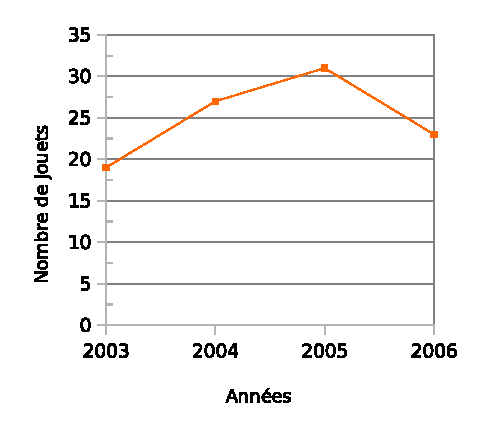
\includegraphics[width=8cm]{graph_entreprise} \end{center}
\begin{enumerate}
 \item En quelle année cette entreprise a‑t‑elle réalisé ses meilleures ventes ?
 \item Décris l'évolution du nombre de ventes de jouets de 2003 à 2006.
 \item Recopie et complète le tableau :
 \begin{center}
  \renewcommand*\tabularxcolumn[1]{>{\centering\arraybackslash}m{#1}}
  \begin{ttableau}{\linewidth}{5}
   \hline
   \rowcolor{J1} Année & 2003 & & & \\\hline
   \rowcolor{J2} \small{Nombre de jouets} & & 27 000 & & \\\hline
  \end{ttableau}
 \end{center}
 \item Combien de jouets ont été vendus de 2003 à 2006 ?
\end{enumerate}
\end{exercice}


\begin{exercice}[Sécurité routière]
Le tableau ci‑dessous donne la répartition, par tranche d'âge, du nombre des victimes dans des accidents dus à l'alcool, en 2007 :
 \begin{center}
  \renewcommand*\tabularxcolumn[1]{>{\centering\arraybackslash}m{#1}}
  \begin{ttableau}{\linewidth}{2}
   \hline
   \rowcolor{C2} Tranches d'âge & Nombre de tués \\\hline
   \cellcolor{U1} 0 ‑ 17 ans & 22 \\\hline
   \cellcolor{U1} 18 ‑ 24 ans & 228 \\\hline
      \cellcolor{U1} 25 ‑ 44 ans & \\\hline
   \cellcolor{U1} 45 ‑ 64 ans & 172 \\\hline
   \cellcolor{U1} 65 ans et plus & 39 \\\hline
   \cellcolor{U1} Âge inconnu & 3 \\\hline
  \end{ttableau}
 \end{center}
\begin{enumerate} 
 \item Le nombre total de tués dans des accidents dus à l'alcool en 2007 est de 966. Recopie et complète le tableau.
 \item Quelle est la tranche d'âge la plus touchée ?
 \end{enumerate}
\end{exercice}



\begin{exercice}[En géométrie]
\begin{center} 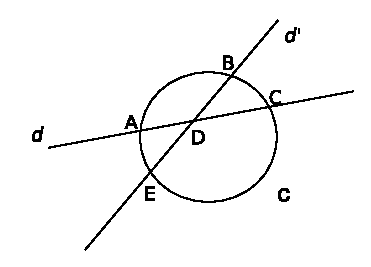
\includegraphics[width=6cm]{tableau_geometrie} \end{center}
\begin{enumerate}
 \item Recopie et complète le tableau par $\in$ ou $\notin$ : \\[0.3em]
  \begin{center}
 \begin{tabularx}{\linewidth}{|c|X|X|X|}
  \hline
   & \cellcolor{F3} Droite $d$ & \cellcolor{F3} Droite $d'$ & \cellcolor{F3} Cercle $\mathcal{C}$ \\\hline
  \cellcolor{H3} A & & & \\\hline
  \cellcolor{H3} B & & & \\\hline
  \cellcolor{H3} C & & & \\\hline
  \cellcolor{H3} D & & & \\\hline
  \cellcolor{H3} E & & & \\\hline
  \end{tabularx}
\end{center}
\vspace{0.5cm}
 \item Construis une figure correspondant au tableau ci‑dessous : \\[0.3em]
  \begin{center}
 \begin{tabularx}{\linewidth}{|c|X|X|X|}
  \hline
   & \cellcolor{F3} Cercle $\mathcal{C}_1$ & \cellcolor{F3} Droite $d$ & \cellcolor{F3} Cercle $\mathcal{C}_2$ \\\hline
  \cellcolor{H3} A & $\in$ & $\notin$ & $\in$ \\\hline
  \cellcolor{H3} B & $\notin$ & $\in$ & $\notin$ \\\hline
  \cellcolor{H3} C & $\notin$ & $\notin$ & $\in$ \\\hline
  \cellcolor{H3} D & $\in$ & $\in$ & $\in$ \\\hline
  \cellcolor{H3} E & $\notin$ & $\in$ & $\notin$ \\\hline
  \end{tabularx}
\end{center}
 \end{enumerate}
\end{exercice}